\subsection{OpenMP}

\subsubsection{Load Balancing}
Initially, the program was parallelized by directingly using OpenMP's loop directive \texttt{for}. By using the \texttt{for} directive, we are allowing OpenMP to handle the distribution of the tasks to the threads. This makes it easier for the programmer; however, it is not the best way to distribute the tasks. For our program, it caused an extreme load imbalance. Upon The distribution of the task was heavily skewed such that the thread with lower id's generated far more combinations than the thread with higher id's. This is because for each element $i$ in the input vector $x$, the number of combinations that can be generated with $x_{i}$ is larger than that with $x_{i+1}$.\\
\null
In order to compensate for the load imbalance, the assignment of tasks to the threads was done in a wrap around manner. Using this method, for the first distribution, each thread will work on the element indexed in the same value as their id (e.g. thread 0 on $x[0]$, thread 1 on $x[1]$, and so on). Then, the following distribution depends on the total number of threads, the id of each thread, and the index of its previous assignment. With \texttt{nth} corresponding to the total number of threads and \texttt{me} corresponding to the thread id, the assignment following the initial distribution is determined using the equation:
\begin{equation}
next\_task = prev\_task + 2 * (nth - me - 1) + 1
\end{equation}
The distribution that will then follow the above depends on the id of each thread the index of the previous task. This next distribution is determined by the equation:
\begin{equation}
next\_task = prev\_task + 2 * me + 1
\end{equation}
The succeeding distributions alternates in using the two equations until the last distribution, which is for $n - m + 1$ or the last $x_{i}$ that can form a combination of size $m$ with the elements succeeding it.\\
\null
In this algorithm, each thread knows which indexes in $x$ to generate combinations for. The threads do not need to communicate with each other, avoiding huge overhead especially for large values of n.

\subsubsection{Chunk Size}
The equations from the section above implicitly defines the chunk size so that each thread gets assigned roughly the same number $x_{i}$'s to work on. It is essentially the number of times task distributions occur in the load balance algorithm, which is roughly $(n-m+1)/nth$.

\subsubsection{Other Performance Tuning Considerations}
\begin{itemize}
\item Cache coherency: Coherence overheads occur when two threads access data on the same cache line even though the variables are not related-an instance called as false sharing. In order to prevent instances of false sharing, the threads are made to work so each will access data that is not altered by any other thread.
\item Synchronization overhead:
\item 
\end{itemize}

\subsubsection{Scheduling Policies}
The load balancing algorithm described in Section 3.1.1 implements a static scheduling policy since the threads are assigned specific tasks and only work on the tasks assigned to them. For the purposes of timing comparisons, additional optional arguments \texttt{sched} and \texttt{chunksize} were added to the function in order to test the speed of the program for the other scheduling policies, namely dynamic and guided. If both arguments are not provided (or set as NULL), the program defaults to the static scheduling policy using the load balancing algorithm. If either dynamic or guided is set, the program uses OpenMP's built-in \texttt{schedule} clause to distribute the tasks to the threads. If the chunksize is not provided, the program sets it to the default chunk size of 1.\\
\null

We performed various tests using the three scheduling policies and experimented with different chunk sizes (for dynamic and guided). It was clear that the load balancing algorithm using static scheduling was the fastest. It eliminates the communication overhead of the dynamic and guided policies since the threads don't have to repeatedly access the task farm for work to, and idleness is still reduced because of the way the tasks are spread among the threads.\\
\null

Therefore, the static method is the one compared to the original function in the next section.

\subsubsection{Comparative Analysis}
The following inputs were used for comparing the speeds of the source code and our OpenMP implementation. OpenMP was run using 8 threads.\\
\null

\texttt{> system.time(combn(c(1:100), 2))}\\
\texttt{> system.time(combn(c(1:300), 2))}\\
\texttt{> system.time(combn(c(1:100), 3))}\\
\texttt{> system.time(combn(c(1:150), 3))}\\
\texttt{> system.time(combn(c(1:200), 3))}\\
\texttt{> system.time(combn(c(1:300), 3))}\\
\texttt{> system.time(combn(c(1:250), 3))}\\
\null

Here are the total number of combinations generated for each test above:\\
\null
\texttt{> nCm(100, 2, 0.10000000000000002)}\\
\texttt{[1] 4950}\\
\texttt{> nCm(300, 2, 0.10000000000000002)}\\
\texttt{[1] 44850}\\
\texttt{> nCm(100, 3, 0.10000000000000002)}\\
\texttt{[1] 161700}\\
\texttt{> nCm(150, 3, 0.10000000000000002)}\\
\texttt{[1] 551300}\\
\texttt{> nCm(200, 3, 0.10000000000000002)}\\
\texttt{[1] 1313400}\\
\texttt{> nCm(300, 3, 0.10000000000000002)}\\
\texttt{[1] 4455100}\\
\texttt{> nCm(250, 3, 0.10000000000000002)}\\
\texttt{[1] 2573000}\\
\null

The elapsed time recorded for each test is the average of three trials. The OpenMP parallelization massively improved the performance of the function. The improvement is invaluable for even bigger inputs (e.g. \texttt{nCm(100, 5)}). The OpenMP implementation still manages to produce an output under 5 seconds, while the original function takes several minutes.\\
\null

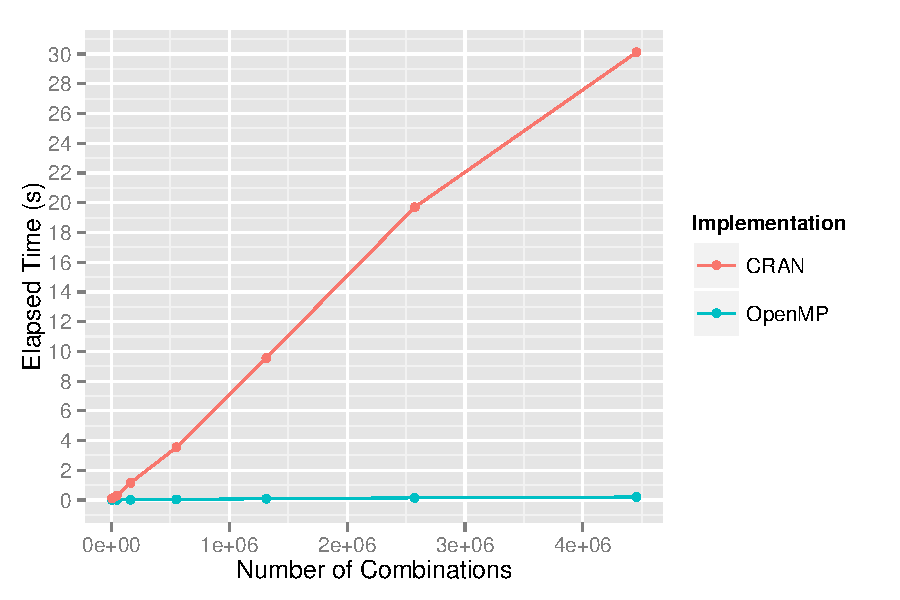
\includegraphics{openmp.pdf}

